% Word limit: 500
\section{Introduction}

\subsection{Gyrochronology}
It has long been known that the rotation periods of FGKM dwarfs increase over
time \citep{skumanich1972}.
This characteristic of main-sequence stars allows them to be dated via their
rotation periods in a practice known as gyrochronology, which is convenient
since the ages of main-sequence stars are extremely difficult to measure via
the traditional age-dating method of isochrone placement.
It is also well established that stars of the same age but different {\it
masses} have different rotation periods \racomment{(citation)}, assumed to be
caused by the deeper convective zones, and therefore stronger magnetic dynamos
(and more efficient magnetic braking) in lower-mass stars
\footnote{Color is the directly observable quantity to which empirical
gyrochronology relation are usually calibrated to, rather than mass or
effective temperature.}.
However, an underlying assumption behind many of the empirical gyrochronology
relations \citep[\eg][]{barnes2003, barnes2007, mamajek2008, meibom2011,
angus2015, angus2019} is that the relationships between rotation period and
color, and rotation period and age are {\it separable}.
In other words, the period-color relation is the same at all ages and the
period-age relation is the same at all colors.
It was recently shown that old stars rotate more rapidly than a simple,
separable gyrochronology relation would predict \citep{angus2015,
vansaders2016, vansaders2018, metcalfe2019}, and that a mass-dependent
modification to the classical \citet{skumanich1972} spin-down law is required
to reproduce the data \citep{vansaders2016, vansaders2018}.
An even more recent analysis of middle-aged open clusters provides further
indication that the exponent of the period-age relation is mass-dependent.
New rotation period measurements of the 1.1 Gyr open cluster, NGC 6811,
revealed a flattened relationship between rotation period and color
\citep{curtis2019}.
In this cluster, the G dwarfs rotate at the same rate as the K dwarfs.

Unfortunately, the open clusters with rotation period measurements are mostly
young -- currently the oldest is 2.5 Gyr (NGC 6819).
Without rotation periods for precisely dated old stars, it is extremely
difficult to calibrate the relationship between rotation period and color at
old ages.
For this reason, we turned to a population-based stellar age indicator,
velocity dispersion, to investigate the period-temperature relations at old
ages.
% Since a separable period-age and period-color relation provided an adequate
% fit for the young stars, it was naturally assumed to apply to old stars too.

\subsection{Kinematics as an age proxy}

Stars are thought to be born in the thin disk of the Milky Way, orbiting the
center of the galaxy with a low out-of-plane, or vertical, velocity ($W$, or
$v_z$).
Young stars have relatively small vertical velocities, but gain momentum in
the vertical direction over time.
Although the cause of orbital heating is not well understood, interactions
with giant molecular clouds are thought to play an important role
\racomment{(citations)}.
Although the velocity of any individual star will only provide a weak age
constraint, the velocity dispersion of a group of stars can indicate whether,
on average, that group is old or young relative to other groups.
In this work we compare the velocity dispersions of groups of stars to
ascertain which groups are older and which younger and draw conclusions based
on the implied relative ages of populations.
% Stellar velocities have a history of being used as an age proxy, with several
% notable examples within stellar astronomy \citep[\eg][]{faherty2009,
% west2011}.
Since the age-velocity dispersion relations (AVRs) are themselves still
actively being calibrated, it is difficult to directly compare gyrochronal
ages with kinematic ones.
However, regardless of the exact relation between velocity dispersion and
stellar age, it is expected to be monotonic relationship, therefore velocity
dispersion can be used effectively to {\it rank} groups of stars by age.
\racomment{Say some words here to prime the reader for the upcoming caveats.}

% Vertical {\it actions} are better age indicators than velocities, because
% actions are calculated by integrating angular momentum over the Milky Way's
% potential, and are therefore position invariant -- \eg\ a star will have the
% same action at periapsis and apoapsis.
% In contrast, orbital velocities are different at periapsis and apoapsis -- so
% in this sense, {\it actions} are the natural quantities to use as age proxies.
Vertical action is a better age indicator than vertical velocity, however both
vertical action and vertical velocity (\vz/W) can only be calculated with full
6-dimensional position and velocity information, yet most stars with measured
rotation periods do not have radial velocity measurements because they are
\kepler\ targets which are relatively faint (between $\sim$11th and $~$18th
magnitudes).
For this reason, we used an alternative age proxy: velocity in the direction
of galactic latitude, \vb.
The \kepler\ field is at low galactic latitude (b=5-20\degrees), so \vb is a
close approximation to \vz.
% Since the stars in our sample only have proper motions, parallaxes and
% positions, with no radial velocites, we could not calculate full 3D velocities
% or actions.

% \subsection{The degeneracy between gyrochronology and mass-dependent heating}

In this paper we tested the \citet{angus2019} gyrochronology relation which
was calibrated using the period-color relation of Praesepe and the period-age
relation of Praesepe and the Sun and is calibrated in \gaia\ \gcolor\ color.
% This relation was calibrated by fitting a 5th-order polynomial to the relation
% between (log) rotation period and (log) \gaia\ \gcolor\ color for around 800
% members of the Praesepe cluster, and a straight line in (log) age to Praesepe
% and the Sun.
Although only calibrated using Praesepe and the Sun, this gyrochronology
relation was tested on NGC 6819, a 2.5 Gyr cluster, for which it predicted
accurate ages
In addition, the period-color relation of Praesepe is nearly identical to the
period-color relation of the Hyades, a cluster of around the same age: $\sim$
650 years \citep{douglas2019}.
However, this relation does {\it not} provide a good fit to NGC 6811, a 1.1
Gyr cluster \citep{curtis2019}.
The G dwarfs in NGC 6811 rotate at the same rate as the K dwarfs and it
appears as though the K stars have `stalled' -- their spin-down has been
halted.
The \citet{angus2019} gyrochronology relation assumes that the rotation
period-color relation of Praesepe is applicable to stars of all ages: the same
polynomial relation fit to Praesepe is used to describe the period-color
relation for all stars.
However, the NGC 6811 cluster suggests that this assumption does not hold past
around 1 Gyr.
If the period-color relation of the \citet{angus2019} gyrochronology model
{\it were} a perfect model for the rotational evolution of stars, then groups
of stars selected to be similar ages using this relation should fall on an
isochrone on both a CMD, and in period-\teff\ space.
Unfortunately, uncertainties on \gaia\ photometry and parallaxes, plus
variations in metallicity and extinction, blur out the main sequence enough
that differences between stars in different age and rotation bins are not
easily discernable on the CMD, although there is still a general age and
rotation period gradient on the CMD, as seen in figures \ref{fig:CMD_cuts} and
\ref{fig:age_gradient}.
For this reason, we chose to use {\it kinematic} `isochrones', instead of
magnitude and color-based isochrones: although kinematics as an age indicator
is not necessarily as well calibrated to an absolute age scale as CMD
position, it can be very sensitive to {\it differences} in the ages of stellar
populations.
\begin{figure}
  \caption{
Main sequence stars with \mct\ rotation periods on the \gaia\ CMD with visual
    binaries removed.
    Points are colored by their gyrochronal age, according to the
    \citet{angus2019} gyrochronology relation.
    A general age gradient is visible across the main sequence.
}
  \centering
    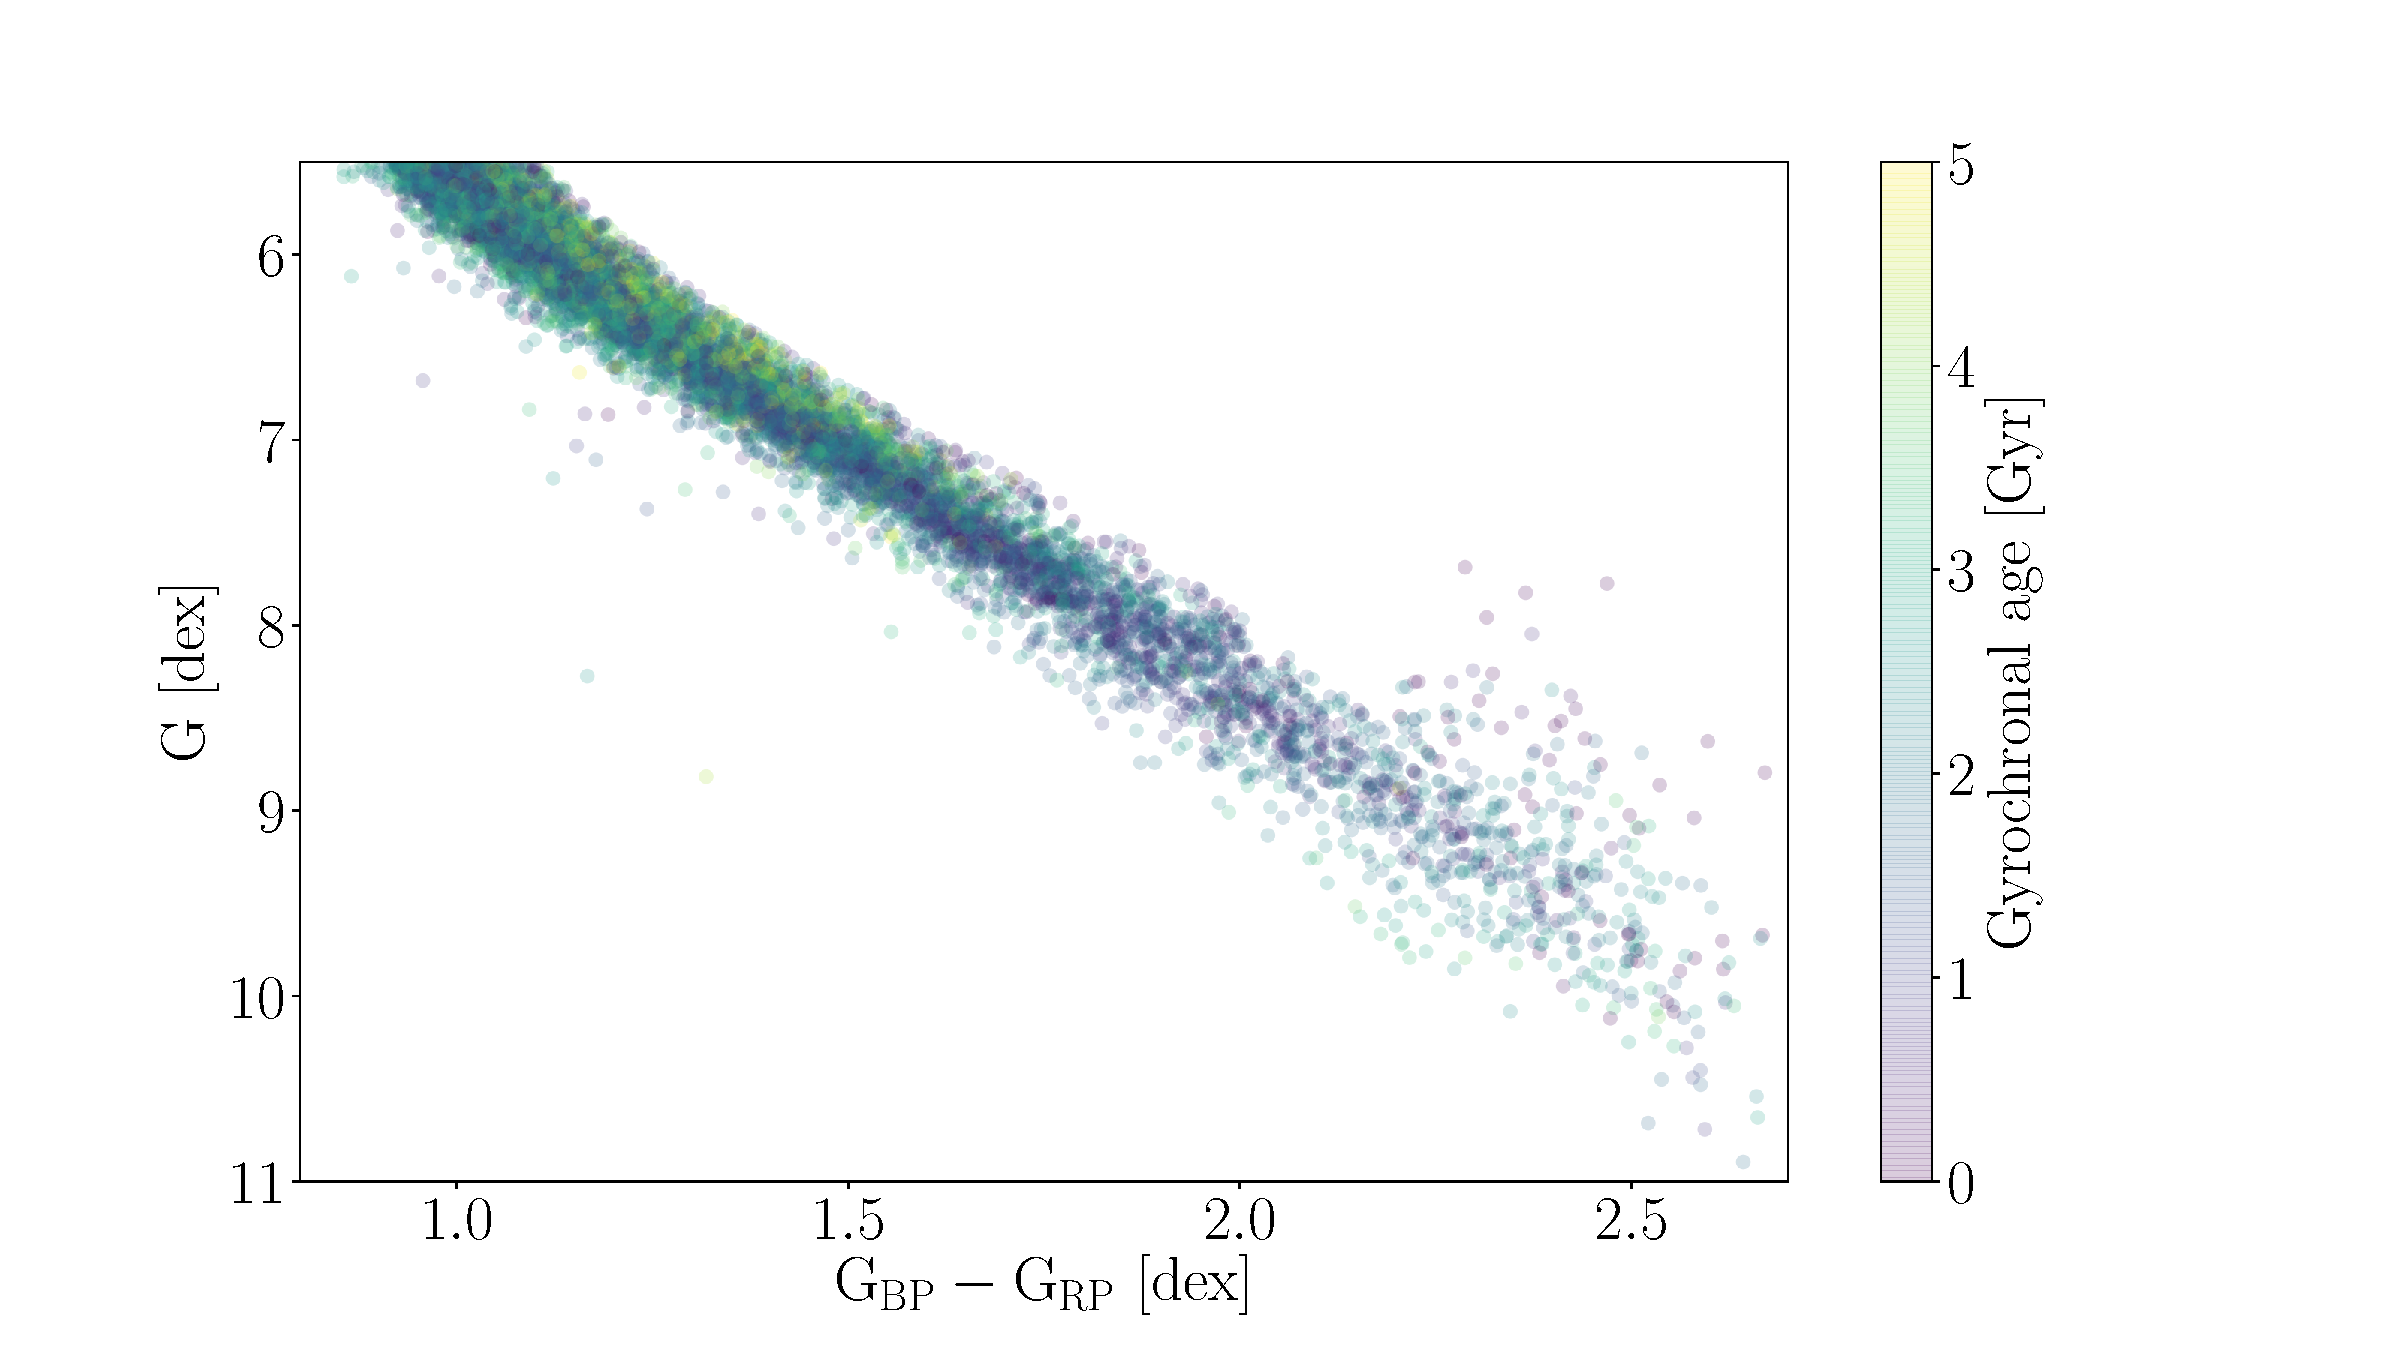
\includegraphics[width=1\textwidth]{age_gradient}
\label{fig:age_gradient}
\end{figure}
Isochrones and stellar evolution tracks are highly dependent on choices made
about input physics and assumptions and have often been calibrated using
different types of stars.
As a result, different sets of models can have very different shapes on the
CMD, particularly at low masses.
Instead of relying on CMD position to age-date groups of stars, we opted to
explore age trends via kinematics.
Kinematic age-dating has the advantage of being relatively model independent,
or at least, having a very simple model: that velocity dispersion increases
over time.
This means that it is relatively easy to rank groups of stars by age: older
groups have a larger velocity dispersion.
It is less easy to rank-order groups of stars by age on the CMD because
stellar evolution is highly mass and metallicity dependent, and because
different stellar evolution models predict different ages for the same CMD
position.
This does not mean that it is not possible to calibrate gyrochronology using
isochrones, however it is not the focus of this study.
